\documentclass[aspectratio=1610]{beamer}
\usefonttheme{professionalfonts}
\usetheme{metropolis}
\usepackage{polyglossia}
\setmainlanguage{german}
\usepackage{amsmath}
\usepackage{amssymb}
\usepackage{mathtools}
\usepackage{graphicx}
\usepackage[
  math-style=ISO,
  bold-style=ISO,
  sans-style=italic,
  nabla=upright,
]{unicode-math}

\setmathfont{Latin Modern Math}

\usepackage{blindtext}
\usepackage{fontspec}
\title[Short version]{Zusatzversuch \\ Untersuchung von Supraleitung}
\subtitle[short version]{A subtitle}
\date{\today}
\author[M. Maier]{Stefan Grisard}


\begin{document}

\frame{\maketitle}


\begin{frame}{Blindtext}
\blindtext

\end{frame}

\begin{frame}{Mehrere Spalten}
\begin{columns}[onlytextwidth]
\begin{column}{0.45\textwidth}
\blindlist{enumerate}[6]
\end{column}
\begin{column}{0.45\textwidth}
\blindlist{itemize}[6]
\end{column}
\end{columns}
\end{frame}

\begin{frame}{oxford Blöcke}
\begin{block}{Erster Block}
\begin{itemize}
  \item hier ein paar Stichpunkte
\end{itemize}
\end{block}
\begin{exampleblock}{Anderer Block}
Hier pipapo
\end{exampleblock}
\begin{alertblock}{Gewagter Block}
Hallihallo, jah f ahd jalkjs aksjd alkjs fgoiho iwqfkalf.
\end{alertblock}
\end{frame}

\begin{frame}{Formeln}
\begin{equation}
  \int_{0}^{1}  (x^2 + 2x)\mathup{d}\, x = \left. \frac{1}{3}x^3 + x^2\right|_0^{1} = \frac{4}{3}
\end{equation}
\begin{equation}
  \int_{0}^{1}  (x^2 + 2x)\mathup{d}\, x = \left. \frac{1}{3}x^3 + x^2\right|_0^{1} = \frac{4}{3}
\end{equation}
\begin{equation}
  \int_{0}^{1}  (x^2 + 2x)\mathup{d}\, x = \left. \frac{1}{3}x^3 + x^2\right|_0^{1} = \frac{4}{3}
\end{equation}
\end{frame}

\begin{frame}{Bilder}

\begin{figure}
  \centering
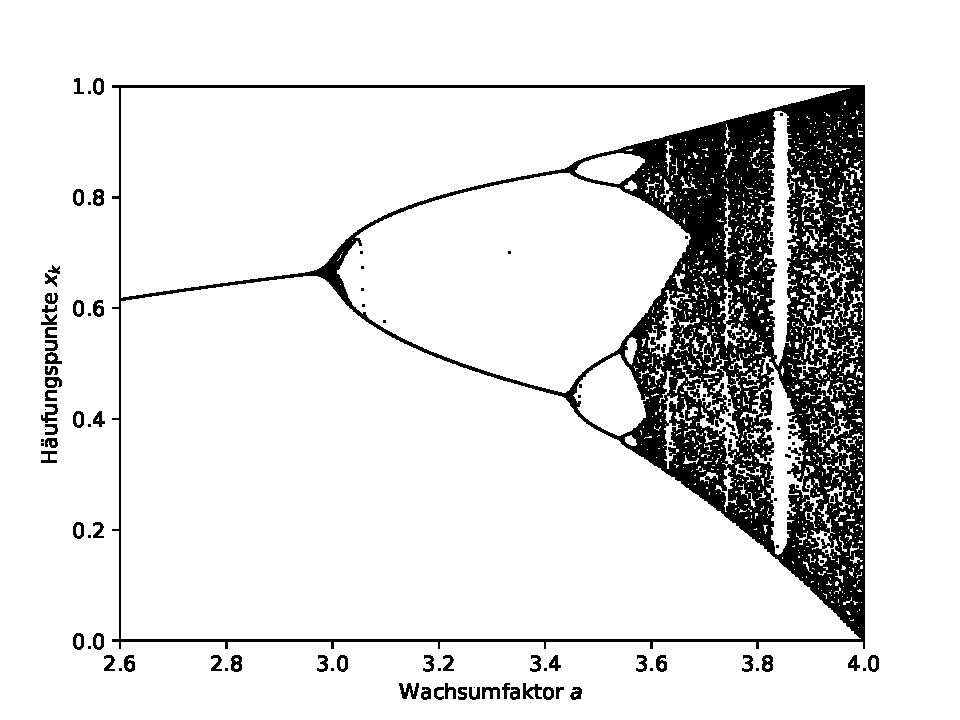
\includegraphics[width=0.7\textwidth]{feigenbaumdiagramm.pdf}
  \caption{TestBild mit Test-Caption}
  \label{fig: testfigure}
\end{figure}


\end{frame}

\end{document}
